\documentclass{CSIM}
\usepackage{enumitem}
\usepackage{subcaption}
\usepackage{cleveref}

\graphicspath{{figures/}}

\begin{document}

% A. Cover Sheet
% A number of the boxes contained on the Cover Sheet are
% electronically pre-filled as part of the FastLane login process
% Complete the rest of your info there

% B. Project Summary
\title{Adaptive Spatial Clustering in Position-Based Dynamics for Real-Time Crowd Simulation}

\newsection{B}




\begin{center}
{\small
\href{mailto:Hkamani@ualberta.ca}{Heena Kamani} \\
\href{mailto:hrho@ualberta.ca}{Hyunsung Rho} \\
\href{mailto:tjongele@ualberta.ca}{Tom Jongeleen}
}
\end{center}

\section{Literature Review}




\subsection{Historical Evolution of Crowd Simulation}

Over the past three decades, crowd simulation research has evolved from macroscopic flow-based approximations to sophisticated multi-agent systems capable of real-time interaction at massive scales. Early approaches emphasized reproducing emergent collective phenomena, while later developments focused on predictive collision avoidance, behavioral realism, and numerical stability under high-density conditions. This progression reflects a gradual shift from aggregate modeling toward constraint-based and adaptive frameworks designed to balance realism with computational scalability.

\subsubsection{Macroscopic and Hybrid}
When it comes to dealing with large-scale crowd simulation, handling collision avoidance is a major challenge. In Continuum Crowds \cite{treuille2006continuum}, macroscopic approach based on continuum dynamics is introduced, where a dynamic potential field integrates global navigation and obstacle avoidance into a single framework. By treating the crowd as a continuous density field rather than individual particles, the model naturally produces emergent phenomena like lane formation and vortices. While computationally efficient, the continuum approach tends to too simplify the crowd, failing to account for individual behaviors and interactions, which can lead to unrealistic results in scenarios where individual decision-making is crucial.

Bridging the gap between microscopic and macroscopic approaches, Narain et al. \cite{narain2009aggregate} introduced Aggregate Dynamics for Dense Crowd Simulation with a dual representation that models the crowd simultaneously as discrete agents and as a continuous system, governed by their unilateral incompressibility constraint (UIC). This allows the simulation to capture the emergent phenomena of large crowds while maintaining individual agent behaviors, providing realistic simulation even with extremely large dense crowds of up to 100,000 agents. However, the approach with UIC simplifies behavioral modeling by optimizing primarily for progress toward desired destinations, which may not fully capture the complex behavioral features observed in real human crowds.

\subsubsection{Microscopic and Adaptive}

Collision avoidance is a critical aspect in crowd simulation. Many early models relied on reactive force-based approaches where agents would respond to the environment and other agents when they were within a certain proximity. However, Karamouzas et al. \cite{Karamouzas2009Predictive} demonstrated that humans anticipate collisions and adjust their paths long in advance. By using a velocity-based approach where agents predict the time to contact, they achieved smoother, more energy-efficient trajectories that avoid the "oscillations" common in earlier reactive models.

\begin{figure}[ht]
    \centering
    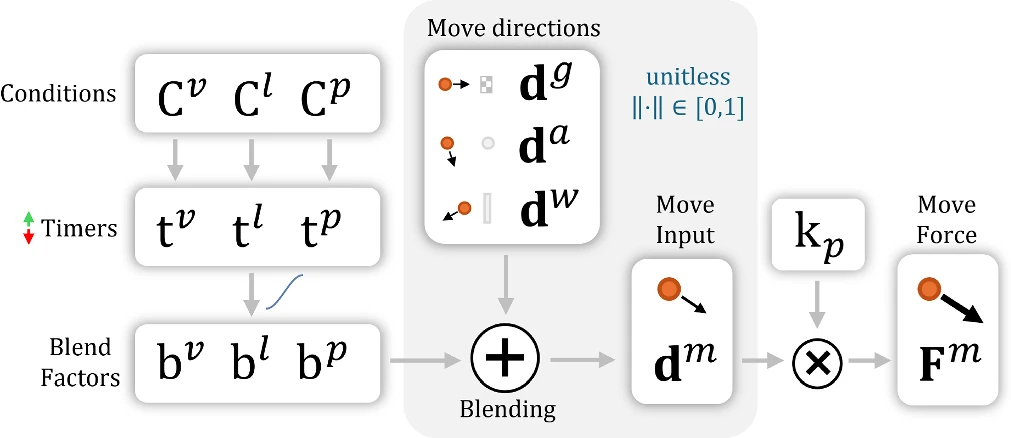
\includegraphics[width=0.5\textwidth]{img/BlendFactor.png}
    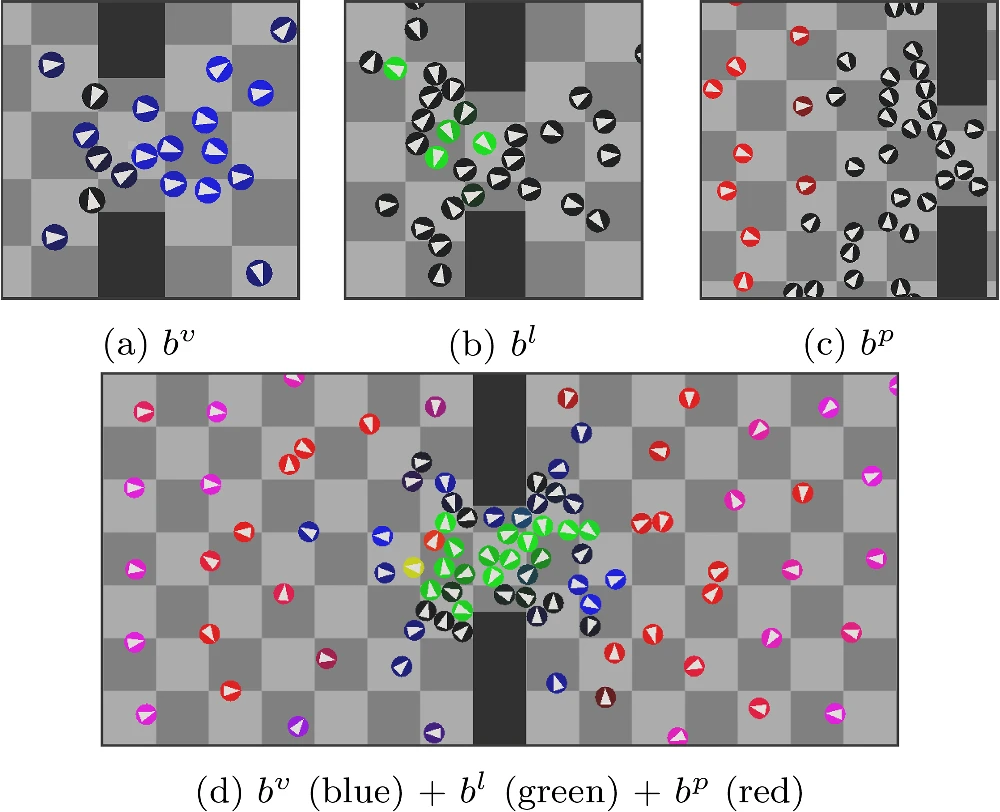
\includegraphics[width=0.5\textwidth]{img/BlendFactor2.png}
    \caption{Adaptive movement behavior in crowd simulation showing context-dependent blending between goal-oriented and avoidance-centric behaviors.}
    \label{fig:adaptive_behavior}
\end{figure}

The recent work by Ruprecht et al. \cite{Ruprecht2024Adaptive}, Adaptive Movement Behavior for Real-Time Crowd Simulation, introduces situational awareness. While earlier models focused on the physics of avoidance, this paper addresses the synthesis of global path planning and local collision avoidance through context-dependent blending. By employing direction-aware neighbor sets and adaptively shifting between goal-oriented and avoidance-centric behaviors, the model allows agents to navigate complex environments with a degree of social and environmental context previously missing from force-based simulations \ref{fig:adaptive_behavior}.


\subsection{Pathfinding in Multi-Agent Systems}

\subsubsection{Partial Refinement A*}

The A* algorithm is a widely used pathfinding method in game development and robotics. However, it can be computationally expensive in large, complex environments. Sturtevant and Buro \cite{Sturtevant2005PartialRefinement} introduced a partial refinement A* that uses map abstraction to create a simplified representation of the environment. This allows for faster pathfinding by first finding a path on the abstracted map and then refining it on the original map. While reducing computational overhead, this method may produce suboptimal paths due to the abstraction.

\begin{figure}[ht]
    \centering
    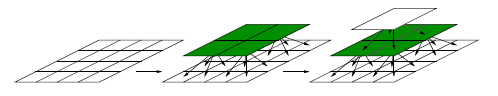
\includegraphics[width=0.8\textwidth]{img/PRA.png}
    \caption{Partial Refinement A* (PRA*) abstraction and refinement process. The original map is abstracted into a simplified representation, where pathfinding is first performed on the abstracted map. The resulting path is then refined on the original map to produce a more accurate route.}
    \label{fig:abstraction}
\end{figure}

\subsubsection{Direction Maps}
Cooperative pathfinding is one of the most significant topics in various fields, including robotics and computer games. The main challenge is from the complexity of the computation, which is often exponential in the number of agents. Direction maps, as proposed by Sturtevant and Jansen \cite{Sturtevant2008DirectionMap}, provide a way to guide agents to cooperate with other agents throughout movement and planning. 

\begin{figure}[ht]
    \centering
    \begin{subfigure}{0.5\textwidth}
        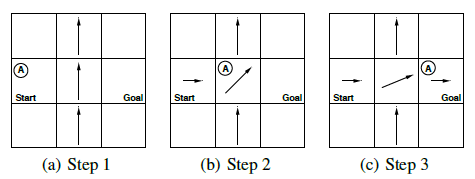
\includegraphics[width=\textwidth]{img/DV.png}
        \caption{Learning Direction Vector}
        \label{fig:direction_map_learning}
    \end{subfigure}
    \begin{subfigure}{0.3\textwidth}
        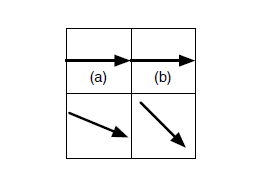
\includegraphics[width=\textwidth]{img/DM.png}
        \caption{Example of Planning with Direction Map}
        \label{fig:direction_map_example}
    \end{subfigure}
    \caption{Direction maps for cooperative pathfinding.}
    \label{fig:direction_map}
\end{figure}

By precomputing a direction map that indicates the encouraged direction for each agent to move based on the current state of the environment and other agents, this method allows for efficient pathfinding in multi-agent systems. Furthermore, in order to further reduce the computational cost, abstraction can be applied to the direction maps, where the environment is simplified into larger regions with uniform direction recommendations \cref{fig:direction_map_abstraction}. This allows for faster pathfinding while still providing effective guidance for agent cooperation.

\begin{figure}[ht]
    \centering
    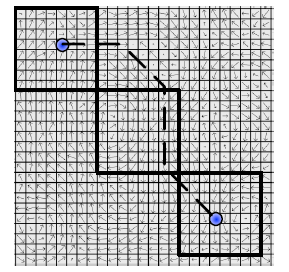
\includegraphics[width=0.25\textwidth]{img/abstraction.png}
    \caption{Abstraction can be applied in direction maps.}
    \label{fig:direction_map_abstraction}
\end{figure}









%
% Section: Collision and Animation in Crowd Simulation
% \section{Collision and Animation in Crowd Simulation}
\subsection{Scalable Interaction and Solver Frameworks}
\label{sec:solvers}

This section reviews key methodologies and recent advances in collision handling and animation strategies for large-scale crowd simulation, with emphasis on approaches that enable real-time performance for dense populations. The discussion synthesizes constraint-based positional methods, velocity-space collision avoidance, perceptual (foveated) animation optimizations, and hierarchical spatial partitioning frameworks that together address the computational bottlenecks of collision dynamics~\cite{weiss,charlton,stancu,sung}.

\subsection{Position-Based Dynamics (PBD)}
Position-Based Dynamics (PBD) has emerged as a robust alternative to explicit force-based schemes for dense crowds, because it enforces non-penetration and other constraints directly in the positional domain rather than through accumulated forces. By iteratively projecting positions to satisfy constraints, PBD mitigates numerical instabilities (e.g., jitter) that commonly arise with large timesteps or high agent densities. Implementations typically combine PBD constraint projection with a lightweight locomotion controller: agent velocities are blended with preferred velocities using an interpolation factor $\xi$ to produce smooth accelerations,
\[
v \gets v(1 - \xi) + \xi v_{\mathrm{pref}},
\]
and neighbor discovery is often implemented with spatial hashing to achieve near-$O(1)$ neighbor queries in practice~\cite{weiss}. PBD's direct position correction provides predictable convergence in high-contact regimes and scales well to tens of thousands of agents when paired with GPU-friendly neighborhood search structures~\cite{weiss}.

\subsection{Velocity-Space Collision Avoidance}
Velocity-space methods, most notably Optimal Reciprocal Collision Avoidance (ORCA), formulate per-agent constraints in velocity space to guarantee (under certain assumptions) locally collision-free motion. The core difficulty for large populations lies in solver scalability: ORCA requires solving small linear programs per agent, and naïve CPU implementations become the $O(n^{2})$ bottleneck as population counts grow. Recent work has focused on migrating ORCA solvers to GPUs using batch linear-program (LP) strategies and careful thread-workload balancing to preserve warp coherency. Grid-based spatial partitioning replaces tree structures in such GPU implementations to provide SIMD-friendly parallelism, memory coherence, and localized queries, producing large speedups (reported up to $\approx 30\times$ compared to optimized multi-core CPU baselines) and enabling interactive update rates for hundreds of thousands of agents under constrained visual fidelity trade-offs~\cite{charlton}.

\subsection{Perceptual Optimization: Foveated Animations}
Animation fidelity often dominates runtime cost when rendering and updating large crowds. Foveated animation leverages human visual limitations—specifically reduced peripheral acuity and the crowding effect—to allocate high-fidelity skeletal updates to the foveal region and progressively coarser representations in the periphery. Typical schemes partition visual eccentricity into zones (e.g., central fovea: full skeletal updates; immediate periphery: reduced update rates but above Critical Flicker Frequency (CFF); deep periphery: statistical or impostor motion only) and adapt update rates to maintain perceived continuity while drastically reducing per-agent animation cost. Empirical prototypes have reported very large reductions in animation operations (orders of magnitude in extreme cases) with minimal perceptual loss when thresholds are chosen based on CFF and eccentricity-dependent perceptual studies~\cite{stancu}.

\subsection{Hierarchical Spatial Partitioning and Rigid-Body Response}
For rigid-body interactions and narrow-phase contact resolution, hierarchical spatial partitioning (e.g., octree combined with AABB pruning) provides an effective defense against quadratic contact-check explosion. A shallow, GPU-traversal-friendly hierarchy—often a two-level scheme—strikes a balance between culling efficiency and traversal overhead. Collision response commonly employs a two-stage strategy: mass-weighted penetration correction (frequently using Baumgarte-style stabilization) to remove interpenetration reliably, followed by impulse-based velocity updates using Coulomb friction models to produce plausible restitution and tangential sliding or sticking behaviors. Such hierarchical frameworks have demonstrated robustness for complex meshes and have enabled interactive rigid-body simulations at scales where flat broad-phase methods fail~\cite{sung}.

%\subsection{Synthesis and Practical Considerations}
%Modern, large-scale crowd systems tend to combine multiple techniques: PBD or constraint projection for close-contact stability, GPU-accelerated velocity-space solvers for locomotion-level collision avoidance, foveated or perceptual LODs for animation, and hierarchical spatial structures for rigid-body culling. Practical system design requires careful profiling of (1) neighbor discovery and spatial data structure traversal, (2) per-agent solver workload balance on the GPU (to avoid warp divergence), and (3) perceptual thresholds that determine where fidelity can be reduced without visible artifacts. The combined approach allows interactive simulation for very large populations provided engineers accept calibrated perceptual and visual trade-offs~\cite{weiss,charlton,stancu,sung}.

\subsection{Geometric Representations of Agents}
\label{sec:geom}

\subsubsection{Disc-Based Models}
Discs are computationally cheap and isotropic; they simplify many algorithms but omit orientation and rotational behavior. The rotational symmetry that makes discs easy to compute is also their limiting factor in narrow passages and close-proximity interactions.

\subsubsection{Ellipse and EOBB Representations}
Ellipses and oriented bounding boxes introduce orientation and better ground-plane approximation at modest extra cost. They improve corridor behavior and reduce conservative collision footprints, but they complicate distance computations and projection formulas.

\subsubsection{Capsule-Based (Torso) Representations multi-agent torso crowds}
\label{sec:torso-crowds}
A recent thread of work shows that explicit torso modeling (2D capsules) captures per-agent rotation, shoulder clearance, and head profile in a simple geometry that aligns closely with human torso footprints~\cite{talukdar2025,stuevel2017}. Talukdar and Weiss (2025) present a PBD-based formulation with three interacting constraint families that directly address close-proximity collisions:

\begin{itemize}
  \item \textbf{Short-range interaction (contact constraint).} Compute the shortest point-pair between two capsule line segments and enforce a non-penetration constraint on the corresponding disc radii extracted from each capsule cross-section. If $\tilde{x}_i,\tilde{x}_j$ are the closest points, the inequality constraint is
  \[
  C(\tilde{x}_i,\tilde{x}_j) = \|\tilde{x}_i - \tilde{x}_j\| - (r_i + r_j) \ge 0,
  \]
  and violation is corrected by the standard PBD mass-weighted projection (see Eq.~(4) in \cite{talukdar2025}). This disc-superposition trick simplifies narrow-phase corrections while preserving the capsule geometry's benefits.
  \item \textbf{Personal-space constraint.} A soft spacing constraint increases comfort distance and invites early maneuvers. Talukdar et al. model it with a per-agent threshold (user-tunable) so that $C(\tilde{x}_i,\tilde{x}_j) \ge d_{\mathrm{personal}}$ and correct violations with reduced stiffness for organic, anticipatory motion.
  \item \textbf{Long-range (anticipatory) interaction.} Using predicted positions along each agent's velocity, future time-to-contact $g$ is computed (as in Weiss et al.), and if $g$ exceeds a configured threshold the algorithm applies softened, timed positional corrections scaled by a stiffness factor $\exp(-\hat{g}^2/g_0)$ to avoid sudden maneuvers. Talukdar et al. adapt disc-based future-collision calculations to capsule pairs using the closest-point projection described above, enabling anticipatory rotation and lane-forming behavior in tight spaces~\cite{talukdar2025}.
\end{itemize}

Beyond constraints, the torso work adds a \textbf{rotation planner} that computes available clearance along the agent's forward axis and derives a target rotation $\theta^\star$ (clamped per time-step) so agents can turn their torso to exploit local clearance (see Fig.~5 in \cite{talukdar2025}). The practical payoff is significant: capsules can pass where discs deadlock, and torso-aware PBD supports smoother close-proximity behavior while remaining amenable to PBD's constraint projection pipeline.


\subsection{Perception and Computational Scalability}
\label{sec:perception}

Real-time crowd simulation remains a central challenge in computer graphics due to the rapidly increasing computational cost of inter-agent interactions as density grows. While substantial progress has been made in geometric modeling, motion realism, and rendering optimization, comparatively fewer works address adaptive reduction of constraint-solving complexity within dense agent clusters. This section examines perception-based strategies in crowd simulation, with particular emphasis on their relationship to computational scalability.

\subsubsection{Perception and Computational Importance}

Perception has been incorporated into crowd simulation in two primary ways: as a cognitive model influencing agent behavior, and as a perceptual optimization mechanism guiding computational resource allocation.

\paragraph{Agent-Centric Perception Models}
Hierarchical perception models integrate visual, auditory, and tactile filtering with memory structures \cite{Sun2008Hierarchical}. In these systems, perception is processed in stages: sensory filtering, short-term memory storage, long-term memory accumulation, and behavioral interpretation.

Research demonstrates that perceptual range varies with crowd density. Occlusion and psychological stress reduce effective sensory range in high-density conditions, influencing navigation behavior and evacuation dynamics \cite{Sun2008Hierarchical}. Selective attention mechanisms prioritize stimuli based on objective features (distance, velocity) and subjective traits (personality, risk tolerance) \cite{Macklin2014Unified, Sun2008Hierarchical}. While such cognitive perception models enhance behavioral realism, they primarily affect decision-making rather than computational complexity within physics solvers.

\paragraph{Viewer-Centric Perceptual LOD}
A separate line of work exploits limitations of human visual perception to reduce computational cost. Perceptual Level of Detail techniques lower geometric or animation fidelity for agents deemed visually less important, often based on distance, screen-space size, or gaze direction \cite{Reddy2001Perceptual}.

Foveated animation approaches allocate higher update rates within the viewer's central field of view and reduce update frequency in peripheral regions \cite{Reddy2001Perceptual}. These techniques yield substantial rendering savings while maintaining perceptual plausibility. However, they predominantly target animation and rendering pipelines rather than the constraint-resolution stage of physics-based solvers. Thus, existing perceptual optimization strategies reduce visual computation but do not directly address the density-dependent growth of constraint-solving cost.

\paragraph{Summary of Perception Research}
Perception modeling contributes to both behavioral realism and perceptual optimization. Agent-centric models introduce cognitive constraints that influence navigation decisions, while perceptual LOD techniques reduce rendering workload based on viewer importance. Nevertheless, current approaches rarely integrate perceptual importance directly into the dynamics layer. In particular, few methods adapt constraint resolution fidelity within physics-based solvers according to perceptual significance.

\subsubsection{Synthesis and Research Gap}

%The preceding review highlights a structural gap in the literature. While PBD provides stable and scalable collision handling, its computational cost remains proportional to local interaction density. Perceptual LOD methods reduce animation and rendering expense but do not reduce the number or complexity of constraint projections in dense regions. Consequently, there is limited exploration of frameworks that dynamically adjust constraint-solving fidelity based on perceptual importance and spatial clustering.
%
%This gap motivates the development of a Computational Level of Detail (C-LOD) framework that integrates Adaptive Spatial Clustering directly into the PBD constraint resolution stage. By clustering agents spatially and modulating constraint fidelity according to perceptual importance, it becomes possible to reduce solver workload in dense regions while maintaining perceptual realism in areas of high visual significance.

We now close the narrative: PBD gives stable, extensible collision handling; torso/capsule geometry resolves many close-proximity artifacts; velocity-space and GPU-accelerated LPs scale locomotion. Yet a persistent mismatch remains — as local density grows the \emph{constraint cost} grows, but perceptual LODs do not reduce solver work. Few methods explicitly tie perceptual importance to the fidelity of constraint resolution. This observation motivates the present work: \emph{Adaptive Spatial Clustering} inside a PBD pipeline, where clusters modulate constraint fidelity according to perceptual relevance and spatial coherence, promising large solver savings while preserving visible realism.



% \newpage\newsection{C}


% % C. Table of Contents 
% % A Table of Contents is automatically generated for the proposal by FastLane

% D. Project Description
% \newpage\newsection{D}
% \input{sections/plan}

% % E. References Cited

\newpage\newsection{C}
\renewcommand\refname{References Cited}




% I prefer to use the IEEE bibliography style. 
% That's  NOT required by the NSF guidelines. 
% Feel Free to use whatever style you prefer
% \bibliographystyle{plain}
\bibliographystyle{IEEEtran}
\bibliography{references}

% % F. Biographical Sketch(es)
% \newpage\newsection{F}
% \input{sections/bio}

% % G. Budget Justification
% \newpage\newsection{G}
% \input{sections/budget}

% %  H. Current and Pending Support
% \newpage\newsection{H}
% \input{sections/support}

% % I. Facilities, Equipment and Other Resources
% \newpage\newsection{I}
% \input{sections/resources}

% % J. Special Information and Supplementary Documentation
% \newpage\newsection{J}
% \input{sections/data}		% Data Management Plan (Required)
% %\input{sections/postdoc} % Postdoctoral Researcher Mentoring Plan (if applicable)

\end{document}

